\documentclass[11pt, oneside]{article}   	
\usepackage{geometry}                		
\geometry{letterpaper}                   		
\usepackage[parfill]{parskip}    		
\usepackage{graphicx}							
\usepackage{amssymb}
\usepackage[utf8]{inputenc}
\usepackage{float}
\usepackage{datetime}
\newdate{referencedate}{07}{11}{2017}

\graphicspath{ {} }

\title{Software Project Management Assessed Exercise One - Domain Document }
\author{Paul McHard - 2085227M}
\date{\displaydate{referencedate}}							

\begin{document}
\maketitle
\tableofcontents
\section{Domain Description}
\subsection{Introduction}
Gaelic TV produce a programme schedule including predicted viewing figures. These figures are drawn from actual viewing patterns which the department receives from a third party. The data they use is stored in a database and shows the figures from the equivalent day approximately one month prior. Currently the scheduling department make schedules using spreadsheets, which are done by hand using commercial spreadsheet packages. These spreadsheets are passed to marketing to identify prime advertising slots which are then sold to advertisers. Human error in predicting viewing patterns is a concern.

The proposed system will automate the process of predicting viewing figures. It will also allow for more rapid and accurate handling of short term changes such as breaking news or major events. Gaelic TV would like for the system to use a drag and drop functionality in creating timesheets. It is also desired that the system should have functionality to generate an optimised timesheet providing the consistently highest viewing figures across a scheduled day.

\subsection{Glossary}
\begin{itemize}
\item \textit{Head of Scheduling}: In charge of department. Has overall responsibility and approves any timesheet before it passes to marketing department.
\item \textit{Scheduling Assistant / Admin}: Head of Scheduling's Assistant, responsible for creation of timesheets.
\item \textit{Timesheet}: A television listing schedule for a given day including predicted viewing figures.
\item \textit{Timeslot}: A position on the timesheet of variable duration into which a programme is allocated.
\item \textit{Viewing Figures}: Can be either actual or predicted. Shows the number of people who respectively either watched or are predicted to watch the channel during any given broadcast.
\item \textit{Watershed}: Regulatory restriction which only allows the broadcasting of adult content between 9pm and 5:30am.
\item \textit{Ofcom}: UK regulatory body on broadcasting and telecommunications. 
\end{itemize}
\subsection{Domain Knowledge}
\subsubsection*{Time Limitations and Live Broadcasts}
Television stations in the UK are bound by regulations regarding the Watershed. Scheduling must pay careful attention to prevent broadcasting of adult content before the watershed, which is 9pm. Additionally Ofcom has guidelines that television stations must follow regarding the transition to adult material post watershed.\cite{ofcomwebsite}

Live broadcasts are regarded with higher scheduling priority than other programmes. These include regular live broadcasts, such as the news, and major live events such as sports games. The station endeavours to broadcast these programmes live as much as possible, and also optionally may broadcast highlights at a later stage as well. Predictions for these are usually made using a separate set of historical data than the usual daily viewing figures.
\subsubsection*{Genre Grouping}
When categorising television shows for broadcast the key descriptor is the programme's genre. Genre is of key consideration to the station during scheduling. Organising a broadcast schedule based on genre can benefit the viewing figures and ratings that the station receives for a given day.
\subsubsection*{Viewing Data Source}
Viewing Figures are received from an external source each day and saved automatically into the station's database. These figures are stored as a spreadsheet. Each day the station will receive the viewing data from that day one month prior. The station has no control over the rate of processing of these figures, nor the style in which they receive them. The data is broken down by demographics: Adult Males, Adult Females and Children. The station assumes the data to be accurate and is not responsible for the accuracy of this information, only the accuracy of its predictions based upon it.
\subsubsection*{Preparation Deadlines}
The station requires that a broadcasting schedule for a given day must be prepared one week in advance. It can be edited at a late stage in the event of breaking news occurrences or other likewise exceptional circumstances.
\subsection{Customers and Users}
The customer for the proposed system is the Scheduling Department of Gaelic TV. The primary users will be the Head of Scheduling and their assistant(s). Customer's Head of IT will have access privileges to update the system, but does not use the system otherwise. The system must automatically pass complete and approved timesheets to Marketing Department but they do not make use of the system directly.
\subsection{Environment}
Gaelic TV has computers and servers which are maintained by its own IT department. Majority of staff use Windows PCs running recent versions of Windows Operating Systems. Some user's make use of Apple Mac or Linux and so the system must be cross platform.
\subsection{Existing Procedures}
The Scheduling Assistant / Admin prepares timesheets. This is done one week in advance for any given day. The current system uses spreadsheets which the Scheduling Assistant prepares by hand. A scheduled day is 15 hours long and must be filled with television shows with slots in between for adverts. These advertising slots are left vacant for marketing to fill. Currently the Scheduling Assistant will estimate viewing figures for a given show at a given time based on previous viewing figures from one month before. These viewing figures are stored in a database which the Scheduling Assistant has access to. 

When the Scheduling Assistant has prepared a timesheet, which contains the programme schedule and predicted viewing figures, it must be approved by the Head of Scheduling. After a timesheet has been approved, it is passed to marketing, who use it to sell advertising slots based on the viewing figures of shows around each advert block. The Head of Scheduling sometimes prepares timesheets, however this is usually if the Scheduling Assistant is ill or otherwise unavailable.

It is common for the Scheduling Assistant to revise and edit timesheets after they are completed due to major events such as live sports broadcasts or breaking news occurrences. These events are determined as being of a high priority, and typically use separate historical data for reference when predicting viewing figures. This separate data is also stored in the database.

\subsection{Competing Systems}
The customer's current system is to utilise commercial spreadsheet packages; these do not provide the desired automation, hence the customer requires the new system. Other television stations, particularly larger ones, will likely have their own internal scheduling systems. Appropriate commercial scheduling software packages are likely to also be available but will be disadvantaged in their broad target audience and are not tailored to the needs of the customer. In this case excessive additional functionality available in commercial packages can be a drawback as it is seen as unnecessary and overwhelming.
\subsection{Similarities with other Domains and Organisations}
The television industry, and its scheduling in particular, is a largely unique domain. Other systems of time based scheduling will not share the same requirements and restrictions as the television industry. Most television stations will however be very similar to one another in their requirements, restrictions and the guidelines they must adhere to in regards to scheduling, as well as their general larger organisational structure. This most likely extends to television stations throughout the developed world in many other countries beyond the UK.

Many other stations will likely already have scheduling systems and software in place, and there are likely many such software packages available commercially. Therefore, while a generic system would be technologically feasible to produce, it might not be commercially or economically viable to do so.
\section{System Non-functional Requirements}
\begin{itemize}
\item System must authenticate users before access granted.
\item User will interface with system via a GUI.
\item System must run on Windows and should be cross platform with Macintosh and Linux.
\item System must have some level of internal network access to reach database and contact Head of Scheduling and Marketing.
\item System must have different privileges based on different levels of security for different users.
\item System must output in the form of a spreadsheet.
\item System must access database via stored procedures and is not granted procedural access.
\item System must not handle back-up and database procedures.
\end{itemize}
\section{Use Cases}
\subsection{Use Case Groupings}
Use Cases are categorised into four divisions: \textbf{Must Have}, \textbf{Should Have}, \textbf{Could Have} and \textbf{Would Like To Have}. These are divided based on their priority in development and the degree to which they are critical to the functionality of the program. The Use Cases of the program are divided as follows:
\paragraph{Must Have}
\begin{itemize}
 \item Create New Timesheet
  \item Edit Timesheet
 \item Commit Timesheet
 \item Get Previous Viewing Data
 \item Approve Timesheet
 \item Receive Timesheet
\end{itemize}
\paragraph{Should Have}
\begin{itemize}
 \item View Previous Timesheet
 \item Create Timesheet Template
  \item Update System
\end{itemize}
\paragraph{Could Have}
\begin{itemize}
 \item Compare Previous Timesheet with True Data
 \item Auto-Generate Regular Shows
\end{itemize}
\paragraph{Would Like to Have}
\begin{itemize}
 \item Generate Optimal Timesheet
 \item Determine Genre Based Quality
\end{itemize}
\subsection{Use Case Diagram}
\begin{figure}[H]
\centering
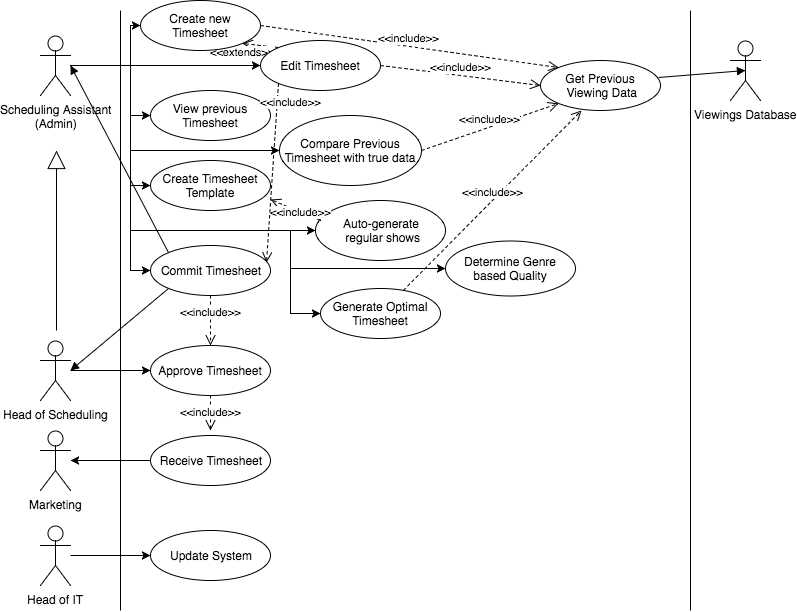
\includegraphics[width=\textwidth]{UseCaseDiagram}
\caption{Use Case Diagram}
\end{figure}
\section{Use Case Detail}
The following section discusses in detail the three Use Cases which are of most significance to the program. The three that are discussed herein are \textit{Create New Timesheet}, which is project critical because it forms the foundation of the project aim, which is to create programme scheduling timesheets; \textit{Edit Timesheet}, which is important as it provides the user the ability to change a timesheet in light of error, breaking news or exceptional circumstances; and \textit{Approve Timesheet}, which is critical as it provides functionality for \textit{Head of Scheduling} to approve a timesheet, and then automatically passes the completed timesheet to marketing.

\subsection{Use Case 1 - Create New Timesheet}
\subsubsection*{Rationale}
\textit{The Scheduling Assistant creates timesheets to schedule programmes and predict viewing figures. This will allow them to create timesheets in a GUI environment where they can add, change and rearrange television shows in a drag-and-drop listing style.}

\textit{The Use Case will actively predict viewing figures, based on previous viewing data, in real time as the user arranges the timesheet. It will inform the user of errors such as adult content pre-watershed and timeslots which are vacant, but is not capable of generating optimised timesheets or informing user of better arrangement then the one proposed}
\subsubsection*{Actors}
The \textit{Scheduling Assistant} is the active actor for this use case.
The \textit{Head of Scheduling} is an active actor by inheritance from \textit{Scheduling Assistant}.
The \textit{Viewings Database} is a passive actor by inclusion of \textit{Get Previous Viewing Data} Use Case.
\subsubsection*{Priority}
This Use Case is \textbf{Must Have}.
\subsubsection*{Status}
Development of this Use Case has yet to commence.
\subsubsection*{Pre and Post Conditions}
There are two preconditions for this use case:
\begin{itemize}
\item The user's login credentials have been verified.
\item No timesheet for the target day exists. 
\end{itemize}
There is one postcondition for this use case: 
\begin{itemize}
 \item The produced timesheet must not contain any null-valued time-slots; every section of broadcasting time within the 15 hour window must be occupied.
 \end{itemize}
 \subsubsection*{Internal Use Cases and Extension Points}
Use Case \textbf{includes} the \textit{Get Previous Viewing Data} Use Case, to retrieve most recent viewing figures from the Viewings Database, which is a passive actor in the use case.

Use Case may \textbf{include} the \textit{Commit Timesheet} Use Case, as this Use Case could be automated, contrary to how it appears in Use Case Diagram. This is a design choice that can be made at a later development stage.

This Use Case has no extension points.
\subsubsection*{Flow of Events}
\begin{enumerate}
\item User creates a new timesheet, specifying the day that the schedule is for.
\item System loads previous viewing data from database through internal use case.
\item For each programme that will appear in the schedule, the user creates a program object which has the name, duration and genre and age restriction specified, as well as whether or not the programme is live. 
\item User drags and drops programme objects on the timesheet to arrange the schedule. System predicts viewing figures in real time for each programme.
\item The user can save and close when the timesheet has been completed with no vacancies.
\end{enumerate}
\subsubsection*{User Interface}
Use Case will use a GUI displaying all timeslots, initially all empty, into which user will create and then drag and drop programmes. Timeslot list will run vertically, with a standard block size indicating an hour of television. Lines within these blocks should indicate advertising points, but these must not interfere with placement of programmes. Height of visual objects representing programmes should vary appropriately based on duration. Programme objects can be moved and rearranged but cannot overlap and should snap to an hour/half hour marker when placed, or snap to end of previous programme if unusual broadcast times are in occurrence.
\subsubsection*{Primary Scenario}
\begin{itemize}
\renewcommand\labelitemi{--}
\item Scheduling Assistant Ron creates a new timesheet for an unscheduled day.
\item The system loads the most recently received viewing data.
\item Ron creates a programme and adds it to the schedule.
\item System matches name to a programme in the viewing figures at the same timeslot and predicts viewing figures accurately.
\item Ron repeats this until the schedule is complete.
\item For each added programme the system finds an exact match in viewing data and is able to make an exact prediction.
\item Ron saves the timesheet and exits.
\end{itemize}
\subsubsection*{Secondary Scenarios}
\begin{itemize}
\renewcommand\labelitemi{--}
\renewcommand\labelitemii{$\circ$}
 \renewcommand{\labelenumi}{(\alph{enumi})}
\item Timesheet for day already exists.
	\begin{itemize}
	\item Inform user, do not create new timesheet.
	\end{itemize}
\item Target day is in the past.
	\begin{itemize}
	\item Inform user, do not create new timesheet.
	\end{itemize}
\item Adult Programme scheduled pre-watershed.
	\begin{itemize}
	\item Inform user, prevent placement of programme in timeslot.
	\end{itemize}
\item Programme at different time from viewing figure data.
	\begin{itemize}
	\item Predict figures by using an offset multiplier.
		\begin{enumerate}
		\item Positive if show closer to peak times than in Viewing Figures.
		\item Negative if show further from peak times than in Viewing Figures.
		\end{enumerate}
	\end{itemize}
\item No name match found in Viewing Figures.
	\begin{itemize}
	\item If show of similar genre available.
		\begin{itemize}
		\item Inform user prediction is not exact.
			\begin{enumerate} 
			\item If same genre show is in same timeslot, predict Viewing Figures based on similar genre show
			\item If programme closer to peak time than show of same genre, use a positive offset multiplier to calculate viewing figures.
			\item If programme further from peak time than show of same genre, use a negative offset multiplier to calculate viewing figures.
			\end{enumerate}
		\end{itemize}
	\item If no show of similar genre available.
		\begin{itemize}
		\item Inform user prediction is weak.
		\item Predict viewing figures based on shows in Viewing Data in same timeslot.
		\end{itemize}
	\end{itemize}
\item User attempts to save and quit while timesheet contains vacant timeslots.
	\begin{itemize}
	\item Inform user timesheet is incomplete.
	\item Prevent user from closing the timesheet.
	\end{itemize}
\end{itemize}
\subsubsection*{Other Requirements}
System must have network access and appropriate privileges to access Viewings Database via stored procedures as directed by customer's internal IT department.


\subsection{Use Case 2 - Edit Timesheet}
\subsubsection*{Rationale}
\textit{The Scheduling Assistant or Head of Scheduling may require to edit a timesheet before it airs. This can either be before or after it has been approved and sent to Marketing. In the former case edits may need to be made on day of creation due to mistakes noticed, changes desired or other factors identified prior to its commitment or approval. In the latter case, short timeframe alterations may need to be made to an already committed timesheet in light of breaking news or otherwise exceptional circumstances.}

\textit{This use case will allow the user to make alterations within the same GUI environment as used for creation, to facilitate rapid alterations to timesheets and real time updates to predicted viewing figures.}
\subsubsection*{Actors}
The \textit{Scheduling Assistant} is the active actor for this use case.
The \textit{Head of Scheduling} is an active actor by inheritance from \textit{Scheduling Assistant}.
The \textit{Viewings Database} is a passive actor by inclusion of \textit{Get Previous Viewing Data} Use Case.
\subsubsection*{Priority}
This Use Case is \textbf{Must Have}.
\subsubsection*{Status}
Development of this Use Case has yet to commence.
\subsubsection*{Pre and Post Conditions}
There are two preconditions for this use case:
\begin{itemize}
\item The user's login credentials are verified.
\item A timesheet for the target day must exist.
\end{itemize}
There are two postconditions for this use case:
\begin{itemize}
 \item The produced timesheet must not contain any null-valued time-slots; every section of broadcasting time within the 15 hour window must be occupied
 \item The edited timesheet must replace the existing timesheet for the target day, a single timesheet for the day must remain.
 \end{itemize}
 \subsubsection*{Internal Use Cases and Extension Points} 
Use Case \textbf{includes} the \textit{Get Previous Viewing Data} Use Case, to retrieve appropriate viewing figures from the Viewings Database, which is a passive actor in the use case, to match the data used in initially creating the timesheet.

Use Case may \textbf{include} the \textit{Commit Timesheet} Use Case. Again, this Use Case could be automated, contrary to how it appears in Use Case Diagram and this is a design choice which can be addressed later in production. Additionally this use case may be included for purposes of automatically re-committing timesheets which have to be edited after being committed due to breaking news or exceptional circumstances.

This Use Case \textbf{extends} the \textit{Create New Timesheet} Use Case to make use of viewing figure prediction algorithm described therein.
\subsubsection*{Flow of Events}
\begin{enumerate}
\item User opens a previous timesheet.
\item System loads viewing figures used for original predictions from database.
\item For each change the user wishes to make, the system will update its viewing prediction in real time.
\item Timesheets can be saved when the user has completed all desired changes.
\item Timesheets which have already been committed prior to editing are placed on high priority and given option to automatically re-commit for approval.
\end{enumerate}
\subsubsection*{User Interface}
Use Case will use a GUI identical to that described for the \textit{Create New Timesheet} use case. The timesheet being loaded will appear as it was at the end of its creation. It will be entirely editable and follow the same process of allowing programme objects to be dragged and dropped to rearrange.
\subsubsection*{Primary Scenario}
\begin{itemize}
\renewcommand\labelitemi{--}
 \item Scheduling Assistant Ron opens a timesheet he completed earlier that day, but has not yet committed.
 \item The system loads the same data from Viewings Database that it had used during creation.
 \item Ron makes some changes to the schedule, which may include rearranging timeslots, renaming programmes, altering duration, genre or age rating.
 \item For each change, the system re-calculates predicted viewing figures by the algorithm described in \textit{Create New Timesheet}.
 \item Scheduling Assistant Ron saves and closes the timesheet.
 \end{itemize}
\subsubsection*{Seconday Scenarios}
\begin{itemize}
\renewcommand\labelitemi{--}
\renewcommand\labelitemii{$\circ$}
 \renewcommand{\labelenumi}{(\alph{enumi})}
 \item Cannot locate timesheet for desired day to edit.
 	\begin{itemize}
 	\item Prompt User to create new timesheet or search for a different day.
	\end{itemize}
\item Cannot access same previous viewing data in database.
	\begin{itemize}
 	\item Inform User of error, access most recent viewing data.
	\end{itemize}
\item Pre-watershed programme changed to adult.
	\begin{itemize}
 	\item Inform User that this is invalid, prevent saving/closing until error resolved.
	\end{itemize}
\item User attempts to move a programme to an occupied timeslot.
	\begin{itemize}
 	\item Prompt user to decide which programme, occupant or new, should be placed in timeslot.
	\item Place chosen programme in timeslot.
	\item Float remaining programme, visible in GUI but not pinned to timesheet.
	\item Inform user of floating programme, allow for rearrangement.
	\end{itemize}
\item User renames a programme to a name which is already used.
	\begin{itemize}
	\item Inform user of duplicate.
	\item Allow operation.
	\end{itemize}
\item Live Sports Broadcast or Breaking News is added.
	\begin{itemize}
	\item Access separate historical data from database.
	\item Predict Viewing Figures using this data.
	\end{itemize}
\item Timesheet has already been committed.
	\begin{itemize}
 	\item Place on high priority and auto-commit for approval.
	\end{itemize}
 \end{itemize}
\subsubsection*{Other Requirements}
System must have network access and appropriate privileges to access Viewings Database via stored procedures as directed by customer's internal IT department.

\subsection{Use Case 3 - Approve Timesheet}
\subsubsection*{Rationale}
\textit{When a timesheet has been committed by the Scheduling Assistant, it is passed to the Head of Scheduling for approval. If he sees no error and approves it, the system will pass the timesheet to Marketing. If he chooses not to approve it, the Scheduling Assistant will be informed.}

\textit{This use case will allow the Head of Scheduling to ensure that Marketing and the Scheduling Assistant are each automatically informed, in the case of an approval or refusal respectively.}
\subsubsection*{Actors}
\textit{Marketing} is a passive actor in this use case.
\subsubsection*{Priority}
This Use Case is \textbf{Must Have}.
\subsubsection*{Status}
Development of this Use Case has yet to commence.
\subsubsection*{Pre and Post Conditions}
There are three preconditions for this Use Case:
\begin{itemize}
\item The timesheet must be complete.
\item The timesheet must have been committed by the \textit{Scheduling Assistant} or the \textit{Head of Scheduling}
\item The timesheet should ideally be for one week in advance. Shorter timeframes are acceptable for exceptional circumstances.
\end{itemize}
There are two postconditions for this Use Case:
\begin{itemize}
\item If the timesheet is approved, the Use Case must call \textit{Receive Timesheet} to pass to \textit{Marketing}.
\item If the timesheet is denied, Use Case must inform \textit{Scheduling Assistant}.
\end{itemize}
\subsubsection*{Internal Use Cases and Extension Points}
This Use Case \textbf{includes} the \textit{Receive Timesheet} Use Case, which passes a completed timesheet to \textit{Marketing} on completion of this Use Case.

This use case contains no extension points.
\subsubsection*{Flow of Events}
\begin{enumerate}
\item User opens a committed timesheet.
\item User reads timesheet.
\item User approves or rejects timesheet.
\item Relevant parties are informed.
\end{enumerate}
\subsubsection*{User Interface}
This Use Case will use a separate GUI from that used in creation and editing of a timesheet. It will present the user with the final outputted spreadsheet that has been committed as non-editable, allowing the user to read the schedule, with two buttons on window's sidebar to approve or reject the proposed timesheet.
\subsubsection*{Primary Scenario}
\begin{itemize}
\renewcommand\labelitemi{--}
\item Head of Scheduling Ron opens a timesheet.
\item He reads it and decides it is error free and acceptable.
\item He approves the timesheet.
\item Use case calls \textit{Receive Timesheet} to pass to Marketing.
\end{itemize}
\subsubsection*{Secondary Scenarios}
\begin{itemize}
\renewcommand\labelitemi{--}
\renewcommand\labelitemii{$\circ$}
 \renewcommand{\labelenumi}{(\alph{enumi})}
 \item Timesheet is rejected
 	\begin{itemize}
	\item Do not call Receive Timesheet.
	\item Inform Scheduling Assistant that timesheet is rejected.
	\end{itemize}
\item Timesheet was auto-committed on high priority.
	\begin{itemize}
	\item If the timesheet is approved
		\begin{enumerate}
		\item Maintain high-priority tag and call Receive Timesheet to send to Marketing.
		\end{enumerate}
	\item If the timesheet is rejected
		\begin{enumerate}
		\item Do not call Receive Timesheet.
		\item Inform Scheduling Assistant that high-priority timesheet requires editing.
		\end{enumerate}
	\end{itemize}
\end{itemize}
\subsubsection*{Other Requirements}
Program must have network access to pass timesheet from Scheduling to Marketing.


\begin{thebibliography}{5}
\bibitem{ofcomwebsite}
Ofcom: What is the watershed?, \textit{Ofcom},
\\\texttt{https://www.ofcom.org.uk/tv-radio-and-on-demand/advice-for-consumers/television/what\-is-the-watershed}
[Last Accessed \displaydate{referencedate}]
\end{thebibliography}
\end{document}  